%
% $RCSfile: model_view_controller.tex,v $
%
% Copyright (c) 2004. Christian Heller. All rights reserved.
%
% No copying, altering, distribution or any other actions concerning this
% document, except after explicit permission by the author!
% At some later point in time, this document is planned to be put under
% the GNU FDL license. For now, _everything_ is _restricted_ by the author.
%
% http://www.cybop.net
% - Cybernetics Oriented Programming -
%
% http://www.resmedicinae.org
% - Information in Medicine -
%
% @author Christian Heller <christian.heller@tuxtax.de>
%

\paragraph{Model View Controller}
\label{model_view_controller_heading}

After having had a closer look at design patterns for persistence
(\emph{Data Mapper}) and communication (\emph{Data Transfer Object}), this
section considers the presentation layer of an application, which is often
realized in form of a \emph{Graphical User Interface} (GUI).

Nowadays, the well-known \emph{Model View Controller} (MVC) pattern
\cite{buschmann,fowler2002} is used by a majority of standard applications.
Its principle is to have the \emph{Model} holding domain data, the \emph{View}
accessing and displaying these data and the \emph{Controller} providing the
workflow of the application by handling any action events happening on the view
(figure \ref{mvc_figure}). This separation eases the creation of applications
with many synchronous views on the same data. Internally, the MVC may consist
of design patterns like:

\begin{itemize}
    \item[-] \emph{Observer} notifying the views about data model changes
    \item[-] \emph{Strategy} \cite{gamma1995} encapsulating functionality
        of the controller, to make that functionality easily exchangeable
    \item[-] \emph{Wrapper} delegating the controller functionality to the
        strategy mentioned before
    \item[-] \emph{Composite} equipping graphical views with a hierarchical structure
\end{itemize}

Some MVC implementations like parts of the \emph{Java Foundation Classes} (JFC)
use a simplified version not separating controllers from their views. The
\emph{Microsoft Foundation Classes} (MFC) C++ library calls its implementation
\emph{Document-View}.

\begin{figure}[ht]
    \begin{center}
        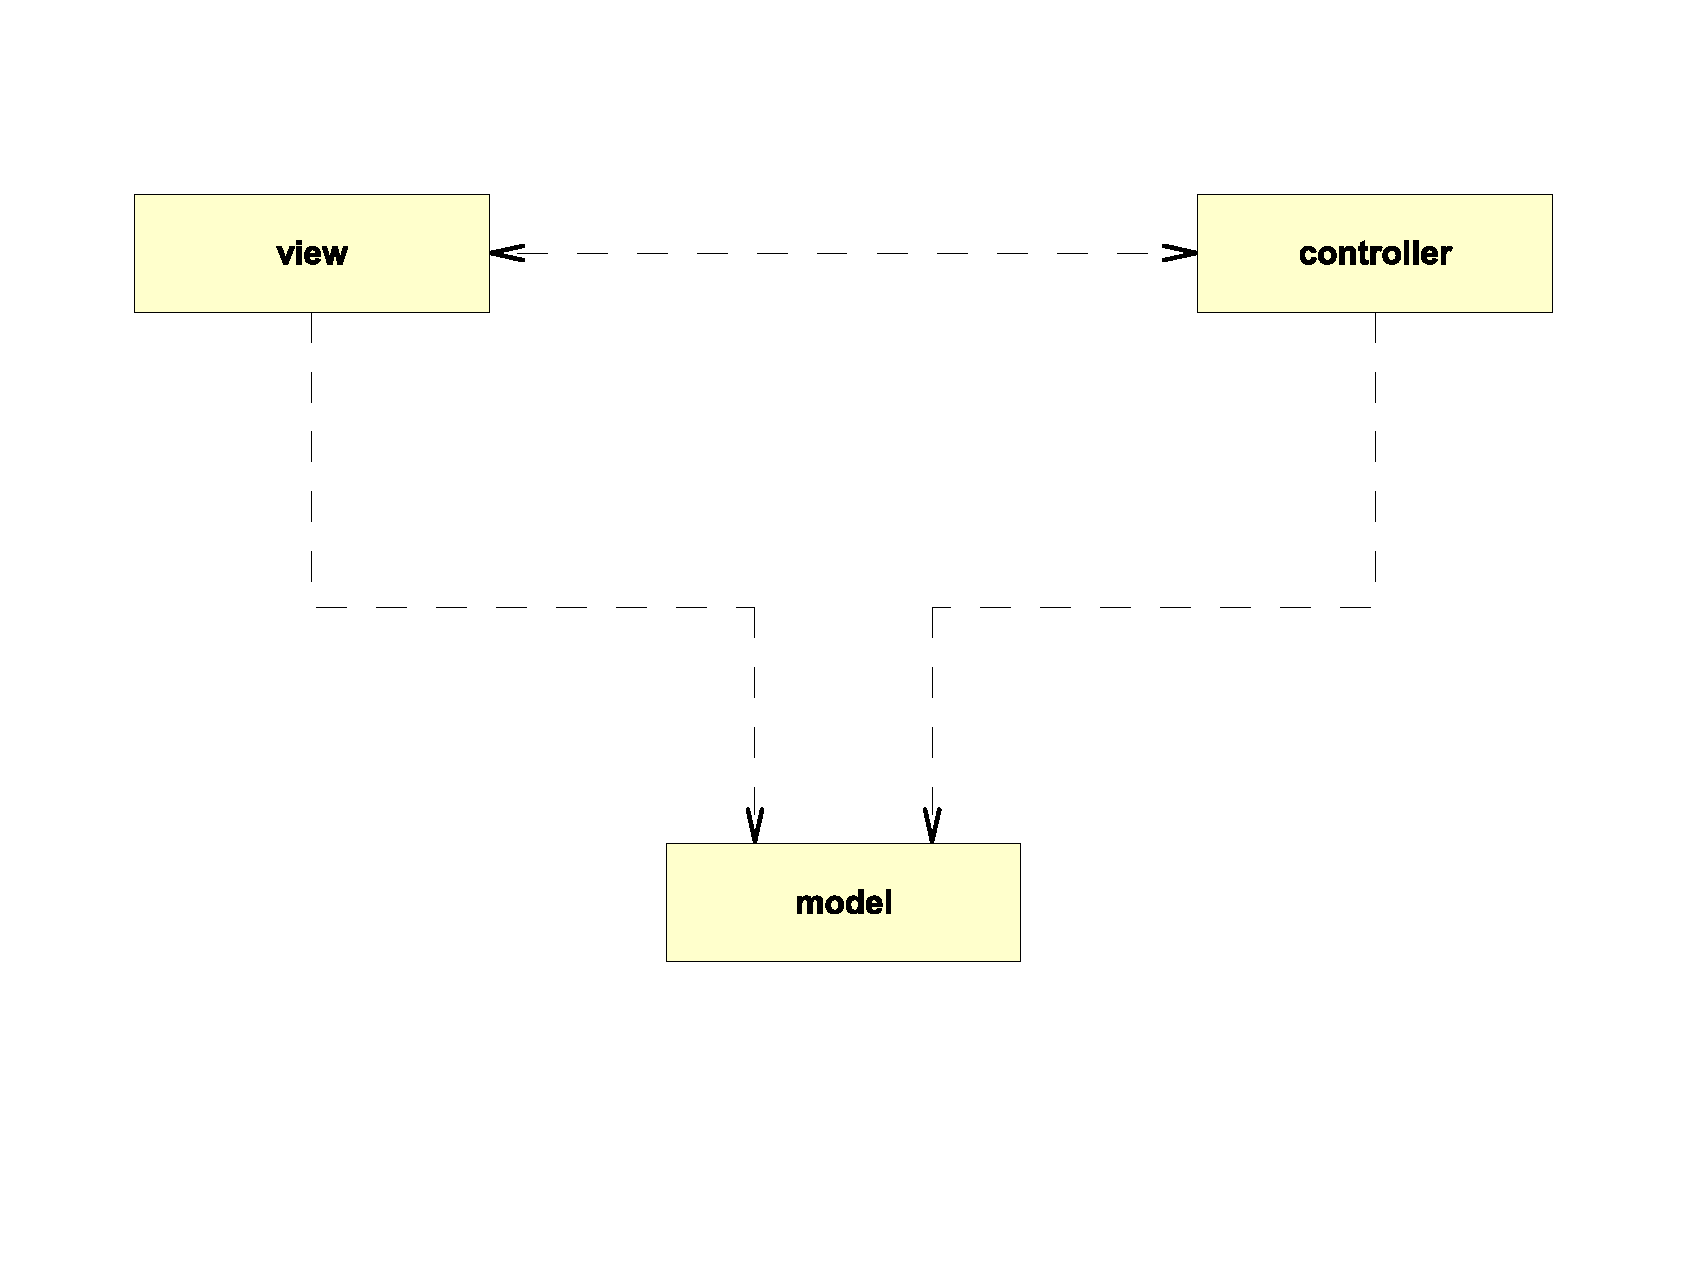
\includegraphics[scale=0.3]{vector/mvc.eps}
        \caption{Model View Controller Pattern}
        \label{mvc_figure}
    \end{center}
\end{figure}
